\documentclass[a4paper,12pt,oneside]{article}

\usepackage{graphicx}
\usepackage{verbatim}
\usepackage{amsmath}
\usepackage[english]{babel} %CHANGER POUR METTRE FRANCAIS
\usepackage[colorlinks,bookmarks=false,linkcolor=blue,urlcolor=blue]{hyperref}
\usepackage{booktabs}

\paperheight=297mm
\paperwidth=210mm

\setlength{\textheight}{235mm}
\setlength{\topmargin}{-1.2cm}
%\setlength{\footskip}{5mm}
\setlength{\textwidth}{15cm}
\setlength{\oddsidemargin}{0.56cm}
\setlength{\evensidemargin}{0.56cm}

\pagestyle{plain}


\def \be {\begin{equation}}
\def \ee {\end{equation}}
\def \dd  {{\rm d}}

\newcommand{\mail}[1]{{\href{mailto:#1}{#1}}}
\newcommand{\ftplink}[1]{{\href{ftp://#1}{#1}}}


\begin{document}

\title{Chaos Déterministe}
\author{Laurent Rohrbasser \& Tim Tuuva}

\maketitle
\tableofcontents
\baselineskip=16pt
\parindent=15pt
\parskip=5pt

\begin{abstract}
%Résumé de l'expérience, on fait des tps sur le chaos, rappeler vite fait 
%dire le but de ces manips, qu'est ce qu'on veut?
\end{abstract}

\section{Introduction}
%expliqué les enjeux théoriques sur le chaos.
%domaine très théoriques
%peu de compréhension sur le sujet ( pourquoi???)

\newpage
\section{Dispositif}
%Description du dispositif expérimental
%Tim's duty
\subsection{Pendule inversé}

\paragraph{Matériels}
%Oui c'est du copier coller je vais voir si je change ca
\begin{enumerate}
	\item Générateur de tension.
	\item Générateur LD Series (A+D Products Bienne Switzerland, EPFL TP physique 466).
	\item Pendule inversé (EPFL TP Physique 41).
	\item Boitier ’Pendule chaotique’.
	\item Boitier SensorCassy (Leybold Didactic Gmbh).
	\item Voltmètre.
\end{enumerate}

\begin{figure}[h!]
  \begin{center}
  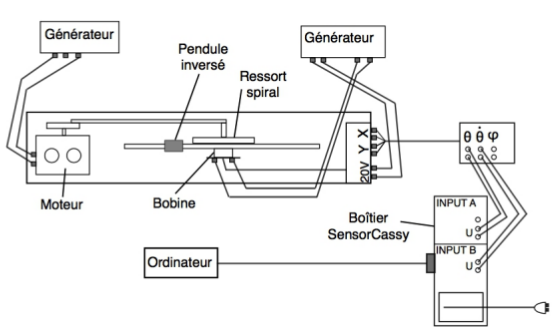
\includegraphics[width=0.5\linewidth,angle=0]{./figures/pendule_inverse.png}
  \caption{Schéma du dispositif du pendule inversé pour le TP sur le chaos déterministe.} \label{fig:pendule1}
  \end{center}
\end{figure}

%TODO PEAUFINER
Le dispositif mesure, grâce au boitier SensorCassy, les valeurs de $\theta$ et $\dot{\theta}$,
permettant de tracer l'espace de phase du pendule inversé.

\subsection{Moteur dipolaire}

\paragraph{Materiels}
\begin{enumerate}
	\item Générateur de fonctions: Wavetek, IPE 241-07/03.
	\item Générateur d’impulsions: EPFL, IPE 242 - 07/03.
	\item Oscilloscope: Hewlett Packard, HP 54600A.
	\item Sonde de Hall : Bell 620 Gaussmeter, IPE 240 - 07/03.
	\item Amplificateur C.C. : EPFL.
	\item Moteur bipolaire : EPFL.
\end{enumerate}

\begin{figure}[h!]
  \begin{center}
  %\includegraphics[width=0.8\linewidth,angle=0]{}
  \caption{} \label{fig:}
  \end{center}
\end{figure}

Un générateur de fonction permet d'envoier un signal triangulaire au
 bornes d'un aimant d'Helmotz, qui va provoquer une perturbation du
 moteur dipolaire. Sur l'oscilloscope, l'entrée X est reliée à une
 sonde de Hall mesurant l'angle $\theta$ du moteur dipolaire via la variation du champ magnétique,
 l'entrée Y est reliée à un électroaimant dont on
 mesure la variation de courant, induit par le champ magnétique
 variant du moteur dipolaire. La fonction trigger est utilisé grâce
 à une sorti sync. sur le générateur de fonction.

\section{Résultats}
%Exposition des graphes avec les légendes et un peu de texte explicatifs sur comment on les a obtenus.

\begin{figure}[h!]
  \begin{center}
  %\includegraphics[width=0.8\linewidth,angle=0]{}
  \caption{} \label{fig:}
  \end{center}
\end{figure}

\section{Discussion}%le plus important

\subsection{Interprétation}
%Qu'est ce que les résultats nous permettent de conclure?
%Est ce que cela nous aide pour nôtre but?

\subsection{Discussions}
%Validité de nos résultats
%S'il y a des erreurs, d'ou viennent elle!
%Avons nous atteind les buts du TP?
\section{Conclusion}

%Résumer du rapport
%Ouverture





%Reference
\begin{thebibliography}{99}
\end{thebibliography}

\end{document}
